\chapter{What's In The Box?}

\begin{wrapfigure}{O}{\figwidth}
	\begin{center}
		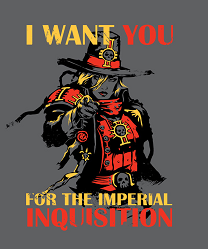
\includegraphics[width=\figwidth]{pics/4/1.png}
	\end{center}
\end{wrapfigure}
This is the ongoing tale of a bunch of guardsmen who got drafted into the Inquisition after their regiment was reduced to a mere 37 men by a combination of Orks, Heretics, more Orks, Tyranids and, of course, their own leadership. 
Currently they work for an Inquisitor that is the 40k equivalent of Professor Oak, he provides teams and missions to Interrogators who need to get some leadership experience before becoming full Inquisitors. 
The lot of these guardsmen is rather thankless, they are matched up with five other less combat focused team members, assigned to an Interrogator, and sent out to fight the enemies of the Imperium.

The squad recently lost their heavy weapons specialist to psyker related bullshit. 
His replacement is Cutter, the only surviving melee specialist from the regiment. 

Cutter is strong, fast, and a little too enthusiastic for comfort. 
He signed up as part of the Regiment's logistical support as a scribe, but the second he got his hands on a Chainsword he found his true calling. 
A life spent scribing followed by a career in swording has left Cutter a little socially inept, but a tendency to scream and hack off limbs excuses most social faux pas. 
His previous squad died rather messily when a bunch of bloodletters got into melee range, only Cutter was equipped to handle a close quarters battle. 
Cutter unsettles the other guardsmen, being bloodthirsty and aggressive is one thing, but willingly leaving cover to close to melee range is just plain crazy.


\begin{wrapfigure}{O}{\figwidth}
	\begin{center}
		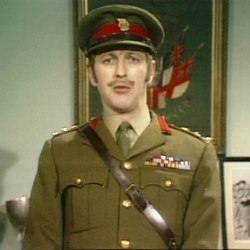
\includegraphics[width=\figwidth]{pics/4/2.png}
	\end{center}
\end{wrapfigure}
Our story starts with the squad taking their seats in the shuttle as their new Interrogator introduces the rest of their team and a briefs them on their mission.
They are being sent to "take a peek at the new poppers some of the lads have found", "make sure everything is tickety-boo with the big hats and the boffins", and "give greeny what for if things get dull". 

A pair of adepts and a pair of tech-priests are trying to figure out what their mission actually is without insulting their new boss. 
An older man is serving tea and helping to decipher some of the Interrogator's more arcane expressions, Doc is taking notes. 
Cutter is ignoring everything in favor of raiding the snack bar and Nubby is picking at the decorative inlay on the table, trying to see if it's actually gold. 
Twitch is watching Sarge and getting very nervous. 
Sarge has realised he is currently in the presence of the greatest known threat to a guardsman's life in the galaxy, an enthusiastic officer.

\begin{wrapfigure}{O}{\figwidth}
	\begin{center}
		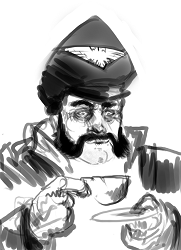
\includegraphics[width=\figwidth]{pics/4/3.png}
	\end{center}
\end{wrapfigure}
So no shit there we were, on our way to an active warzone to investigate some guardsmen's shiny new guns. 
Guns which were apparently so good that soldiers were refusing orders from the Commissariat to destroy them and demands from the Adeptus Mechanicus to fork them over. 
For the sake of these guns guardsmen were actually defying two organizations that scared the bejeezus out of any sane soldier, including us. 
We were quite possibly going to try to TAKE these guns away from an unspecified number of guardsmen. 
While they were using them. 
In the middle of a battle. 
With orks. 
Our Interrogator insisted it would be "jolly good fun".

The Interrogator was such a stereotypical upper-crust officer that it bordered on parody. He was prim, proper, cheerily bloodthirsty, and almost impossible to understand. 
Given the slightest motivation he would regale anyone around him with old war stories, or musings on the art of war, or lectures on proper gentlemanly behavior. 
He wasn't one of the sneering, bureaucratic officers though, he firmly believed he was "just one of the lads" and liked to "get stuck in with the rest of the boys".
To top this all off he actually embraced the moniker Rupert, the insulting guardsman term for a nobby officer, and insisted we call him by it. 
We would have called him that anyways, he was a complete bloody Rupert, but it just wasn't the same if he liked the name.

\begin{wrapfigure}{O}{\figwidth}
	\begin{center}
		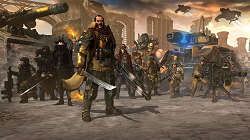
\includegraphics[width=\figwidth]{pics/4/4.png}
	\end{center}
\end{wrapfigure}
He'd spent decades in the Guard leading heroic charges by day, hosting formal dinners during the evening, and retiring to the best accommodations around for the night (fighting in the dark would be "simply barbaric", and was well beneath him). 
At some point in all this he acquired an incredibly skilled batman who became absolutely key to the smooth running of his life. 
Providing tea before it was asked for, scheduling meetings that no one knew was needed, and identifying and disposing of several discrete threats to his charge's life.

One day an Inquisitor took note of the batman's literally supernatural talent for butlery and there was a bit of a scandal. 
One thing led to another and both of them wound up joining the the Inquisitor's retinue. 
Now years later they were still together and working to bring a better class of manners to the Inquisition. We called the batman Alfred.

\begin{wrapfigure}{O}{\figwidth}
	\begin{center}
		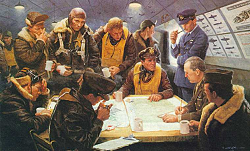
\includegraphics[width=\figwidth]{pics/4/5.png}
	\end{center}
\end{wrapfigure}
We traveled on a Navy vessel in surprising comfort, apparently the Captain's family knew the Rupert's or something. 
In fact it seemed that everyone over a certain rank had some sort of familial connection to our Interrogator. 
The adepts spent the trip learning military law, the tech-priests studied the technical reports on the new guns, and we tried our best to do our usual drill and sleep routine. 

Our Interrogator wouldn't have any of that though, the bugger insisted on wandering down to our barracks every few hours. 
Not a day would go by without him telling us the story of some incredibly valiant charge, stalwart defense, or duel to the death with the enemy's leader. 
Sarge noticed that these stories never seemed to mention how many guardsmen died along the way.

The Rupert also frequently dragged the adepts and tech-priests down to our quarters and insisted they brief us on the results of their research. 
At first we dismissed this as some sort of misguided attempt to build camaraderie in the team, but he kept doing it. 
He even started asking for our opinions and actually listening to them, so long as they didn't go against his own. 
This sort of behavior worried us, it just wasn't normal. 
Something was seriously wrong when the backup muscle gets this much attention and intel.

\begin{wrapfigure}{O}{\figwidth}
	\begin{center}
		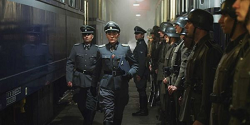
\includegraphics[width=\figwidth]{pics/4/6.png}
	\end{center}
\end{wrapfigure}
Then one day Alfred showed up with perfectly fitted, insignialess dress uniforms for all of us and started lecturing us on how to interact with senior officers as nominal equals. 
With dawning horror we realized that this time we weren't the backup muscle for the adepts and tech-priests, they were the backup brains for us. 
We were the primary investigation team, the Rupert expected us to go and be inquisitive. US, the guardsmen, the mudfeet; a group of under-educated, over-armed gorillas with a penchant for laziness, petty theft, paranoia, and completely reasonable cowardice. 
We were expected to go out there and talk with Imperial Guard Generals, Mechanus Magi, and bloody Commissars, and look for heresy. 
Which we would presumably find by asking these scary people very nicely if they were heretics.

Sarge went spare. 
As a unit our previous experience in this sort of thing consisted of shooting anything we were told to, or was trying to kill us, or just looked weird; we were not qualified to figure this shit out for ourselves. 
Sarge and Doc might have been reasonably intelligent within their fields of expertise, but Nubby was a cretin and a thief, Cutter was borderline psychotic, and Twitch had spent the last few days wiring trip mines into all the cabin's air vents;
 just in case the Navy tried to kill us all in our sleep. 
Of course every time the the subject was broached with the boss-man all it got a was a laugh, an admonition to be more confident, and a story about how good ol' guardsman know-how had solved problems no one else could figure out.

When we finally reached our destination and marched out of our shuttle we were probably the most nervous looking men to ever wear such sinister uniforms. 
If the Rupert hadn't led the way we would have probably been arrested for impersonating officers.

\begin{wrapfigure}{O}{\figwidth}
	\begin{center}
		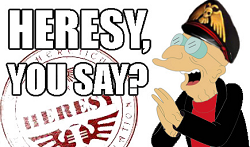
\includegraphics[width=\figwidth]{pics/4/7.png}
	\end{center}
\end{wrapfigure}
The Emperor forsaken ball of dirt we landed on was currently in the grips of a major war with the Orks. 
The planet was being reclaimed from the greenskins, and after the navy had their fun it fell to the guard to remove the Orks from the 'economically vital' regions of planet. %TYPO orks -> Orks
Hundreds of regiments were simultaneously clearing every hive in on the planet with mixed amounts of success. 

One front in particular was doing far better than expected, largely due to the sudden appearance of new more effective weapons in several of its regiments.
Imperial forces were rapidly pushing greenskin forces out of the outer hive, and at this rate the hive would be taken months ahead of schedule. 
Of course the immediate response to such resounding success was the generals on the other fronts calling the Commissariat and Ad-Mech down on the poor suckers. 
Bloody stupid brass.

We walked into a threeway argument between the Commissariat, the Adeptus Mechanicus, and the Generals in charge of the front. 
The Commissars saw guardsmen winning fights without anyone being executed for cowardice, and decided that this was obviously some form of heresy. 
The Ad-Mech saw weapons that were far too shiny for guardsmen to use, and decided that all these guns and their source should be given over to them. 
The front's Generals saw a chance to be big damned heroes, and wanted the Commissariat and Ad-mech to go bother someone else.

\begin{wrapfigure}{O}{\figwidth}
	\begin{center}
		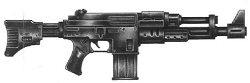
\includegraphics[width=\figwidth]{pics/4/8.png}
	\end{center}
\end{wrapfigure}
Over the next few days we followed our Interrogator around as he talked to seniors officers. 
Our days consisted of meetings, teas, briefings, and formal dinners.
The Rupert seemed to know everybody who was anybody, he constantly chatted with important people while we hung out with their subordinates.

We finally got a clear set of details on the problem at hand. 
Autoguns, chainswords, and body armor that were far superior to standard issue gear was being traded via the guard's black market. 
Guardsmen were quickly trading out their kit for the new gear, and using it to wreck the Orks' shit. %TYPO orks' -> Orks'
The amount of gear that was appearing was as impressive as its quality, but despite the sheer volume of weapons appearing on the market, no one was sure where they came from. 
After all, the Imperial Guard's black market has experience dealing with hostile investigations and both the soldiers and their officers were being less than helpful.

Being a bunch of guardsmen ourselves we weren't inclined to take useful weapons away from soldiers who needed them. 
In our opinion the Commissariat and Ad-Mech were a bunch of dickheads, so we'd only do what they wanted if the weapons or their source proved to be evil. 
So the big questions we needed to answer were: 
What was so special about the guns, did they do anything to the troopers who used them, and where the hell did they come from?

\begin{wrapfigure}{O}{\figwidth}
	\begin{center}
		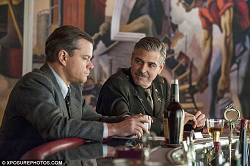
\includegraphics[width=\figwidth]{pics/4/9.png}
	\end{center}
\end{wrapfigure}
Answering these questions was apparently our job, the Rupert seemed to have no intention of doing anything aside from having tea with the rest of the brass.
Occasionally he'd offer a piece of incomprehensible advice, or send us to talk to someone specific, or politely yell at someone who was being difficult, but mostly it was just tea. 
Alfred was generally more helpful, his advice and warnings helped immensely and kept us from making a complete hash of things.

In addition to the dinners, teas, and soirees over the next few days each of us went to a few briefings held by each of the three major players. 
We'd pair up with one of the adepts if we needed legal or investigative advice, or a cogboy if there was going to be any sort of techno-babble. 
Otherwise we'd bring a squadmate for moral support or to act as a lookout if we were doing something sketchy. 
All in all our investigations turned out far better than we had expected. Of course we had expected a complete and utter disaster, so only a few major screwups was considered a wild success in our book.

\begin{wrapfigure}{O}{\figwidth}
	\begin{center}
		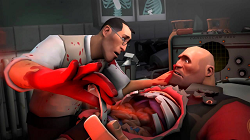
\includegraphics[width=\figwidth]{pics/4/10.png}
	\end{center}
\end{wrapfigure}
The Commissariat and the Mechanicus had detained a few troopers who had been using the weapons and obtained a few corpses of soldiers that had died using them.
The detainees were being kept around for questioning, but the corpses had been immediately cut apart in the name of science. 
As the only member of our team with medical training Doc was sent to talk with the medical staff and magos biologis about what they had found.

Of course Doc wasn't really a doctor, he was a medic. 
He wasn't really in the business of curing people, just making them more comfortable while they die. 
So he thoroughly embarrassed himself during the briefings by asking stupid questions about how to spell things, why a procedure was done, and what the 'green wobbly bit' was. 
In the end though, he managed to determine that none of the soldiers had shown any sign of physical change aside from being a little stronger than average.

Cutter and Sarge went to talk to the Munitorum, since Cutter was a former Munitorum scribe and Sarge didn't trust Cutter not to kill anyone if left alone.
Cutter's scribe training came through and both of them got access to the records the Munitorum kept on the new weapons, as well as a chance to examine one of the chainswords which had fallen into their hands. 
Throwing caution to the winds Cutter took the sword and started swinging it around like an idiot.

Cutter declared the sword to be pretty damned awesome and immediately claimed it as his own. 
When the Munitorum objected he insulted their filing system and challenged them to a duel to the death for ownership of the shiny new sword. 
Sarge considered this to be perfectly normal behavior for Cutter, dumped the problem on one of the adepts, and got Cutter the hell out of there before he killed anyone.

The real problems were Twitch and Nubby, before the end of the investigation both of them were banned from investigating anything ever again.

\begin{wrapfigure}{O}{\figwidth}
	\begin{center}
		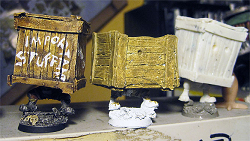
\includegraphics[width=\figwidth]{pics/4/11.png}
	\end{center}
\end{wrapfigure}
Twitch wasn't the most stable person at the best of times, but he was far worse around Orks. 
It was an Ork Kommando raid which had initially triggered his paranoia, so being this near an entire army of them made Twitch incredibly, well, twitchy. 
He was initially sent to interview a few soldiers who had used the mysterious guns. 
Unfortunately each session devolved into him questioning everyone in sight about the last Ork sighting, the quality of the perimeter defenses, and whether anyone else had seen that barrel over there move. 

Twitch's only contribution to our investigation was repeatedly insisting that this was all the Orks' fault.
We eventually gave up on him and let him secure the base after a particularly memorable formal dinner. 
In a short period of time he accused several officers of 'acting orky', decked a clerk who tapped his shoulder, and accused the troopers who restrained him of being cleverly disguised Orks.

\begin{wrapfigure}{O}{\figwidth}
	\begin{center}
		
\includegraphics[width=\figwidth]{pics/4/12.png}
	\end{center}
\end{wrapfigure}
In some ways Nubby was even worse. 
While Twitch wildly accused people and random objects of being Orks in disguise, Nubby was actually mistaken for a gretchin on three separate occasions. 
The first two were embarrassing for everyone involved, but guards are meant to be suspicious and no one was actually hurt. The third time was much worse.

Nubby was supposed to be attending a demonstration of one of the mysterious guns along with one of the tech-priests. 
The demonstration was held in an ad-mech warehouse; 
Nubby being Nubby he immediately dumped the job onto the tech-priest and wandered off to see what was in stock. 
He was found by a pair of servo skulls as he pillaged fancy looking data slates out of several inadequately secured storage lockers.

A short firefight ensued, which attracted a nearby enginseer, who in turn misidentified Nubby as a gretchin looter and called for reinforcements. 
By the time word got to Sarge several more servo skulls were destroyed, Nubby was hiding behind a crate of plasma weapons, and a guard patrol was arguing with the enginseer about whether a gretchin could actually detonate a plasma weapon. 
Sarge sorted everything out and a suspiciously bulky looking Nubby was escorted out of the building in exchange for a promise that he never return.

\begin{wrapfigure}{O}{\figwidth}
	\begin{center}
		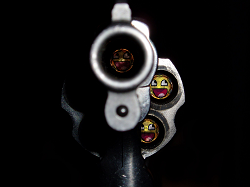
\includegraphics[width=\figwidth]{pics/4/13.png}
	\end{center}
\end{wrapfigure}
Between the interviews and the demos we got a pretty good look at the weapons and their effects. 
The tech-priests said there wasn't anything sinister about their function, they were just very well made and never seemed to jam or misfire. 
There were a lot of fancy words about alloys and mechanisms and shit too, but that really didn't concern us. 
All we knew was that the autoguns hit about as hard as a bolter, the recoil was just hard enough to let you know the gun worked, and both their report and action sounded awesome. 
Cutter expressed similar sentiments about his new chainsword along with dire threats against anyone who tried to take it away from him. 
He did the same thing if you tried to take away his food though, so we were pretty sure it wasn't anything sinister.

The incredible awesomeness of these weapons was suspicious, but Doc was positive that they weren't mutating anyone. 
Just to be sure we had the adepts and Alfred, who we were pretty sure was psychic, see if they could detect anything spooky about the gear. 
None of them detected any warp stuff around the weapons or armor, though Alfred said they were definitely a little weird. 

We had almost all the information we needed now. We knew that the weapons were suspiciously awesome and the soldiers used them because they were awesome. 
We knew that none of the troopers were turning into daemons or mutating and that the weapons weren't doing anything warpy, and Twitch knew that everyone was secretly an Ork. 
The only information that was still missing was the source of the gear, and as it turned out that last piece of intel was in Nubby's pants.

\begin{wrapfigure}{O}{\figwidth}
	\begin{center}
		
\includegraphics[width=\figwidth]{pics/4/14.png}
	\end{center}
\end{wrapfigure}
During his little escapade in the Mechanicus warehouse Nubby had crammed his packs, pockets, sleeves, and pants with expensive looking knick-knacks, parts, tools, and data slates. 
It was standard procedure to hold Nubby upside down and shake him after one of his adventures; 
mostly to see if he had gotten his hands on anything important, but also because we had a running bet on how much he'd take. 
One of several data-slates he had shoved down his pants contained information about a crazier than usual magos who had built a portable weapons factory. 

The factory had provided millions of weapons and tons of ammo to the local PDF, but had stopped working a few years after the magos died to techno-bonitus or something. 
Eventually the weapons were replaced with more standard gear, but the factory was studied by generations of tech-priests hoping to get it working again. 
Right up until an Ork Waaagh rolled over the planet.

We brought this info to the Rupert, who immediately recalled tales of an unusually well armed group of greenskins that had been wiped out recently, as well as the name of the regiment which led the final attack. 
This just so happened to be the same regiment which was spearheading the current attack. 
A few transports were requisitioned and our little force headed out into the thick of things to have a chat with the regiment. 
Of course within minutes of our departure, convoys from the Commissariat and the Adeptus Mechanicus rolled out as well.

\begin{wrapfigure}{O}{\figwidth}
	\begin{center}
		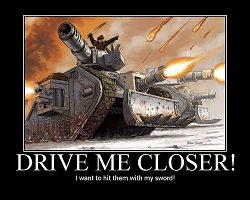
\includegraphics[width=\figwidth]{pics/4/15.png}
	\end{center}
\end{wrapfigure}
The regiment in question was currently so far forward that you had to cross through Ork controlled territory to reach them. 
The only reason they weren't considered to be cut-off and surrounded was the fact that they were kicking so much ass that their boots had started to smell like Ork butt. 
None of us were keen on crossing the gap between the main lines and the regiment, except for the Rupert, who was happily standing out of the top hatch and waving his sword around. 
We were paragons of bravery when compared to the adepts and tech-priests though, they didn’t see the attraction of driving through a burned out city filled with Orks.

The second we left imperial lines our vehicles started taking small arms fire. 
Our Interrogator cheerily blasted away with the pintle mounted gun while we kept our heads down and the non-combatants pissed themselves in terror. 
All in all the drive was pretty pleasant though, nothing heavy enough to pierce the armor was fired at us, the drivers dodged all the land mines, and none of the Orks were good enough shots to hit the Rupert. 
Unfortunately it came to an end at a crude barricade a few blocks short of the regiment's position.

Now a sane man would have just driven back a bit and tried a different street, but not our Rupert. 
With a 'Tally Ho' he hopped out of the top hatch and charged the barricade. 
We all stared at him for a few seconds as he calmly climbed the barricade, completely ignoring the shots landing all around him. 
We were considering the merits of just leaving him out there when Cutter revved his sword and charged after him with Alfred close on his heels.

\begin{wrapfigure}{O}{\figwidth}
	\begin{center}
		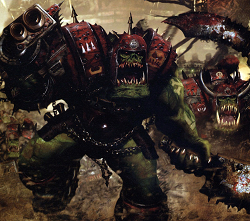
\includegraphics[width=\figwidth]{pics/4/16.png}
	\end{center}
\end{wrapfigure}
No one could call what followed a heroic charge, it had more in common with a comedy sketch than a valiant assault on enemy lines. 

Your typical heroic charge doesn't have two adepts screaming like little girls, or a pair of tech-priests bitching about illogical behavior, or a bunch of guardsmen trying to keep the nerds down below the covering fire from our drivers. 
Also, most charges are supposed to be against something more fearsome than a bunch of Gretchin with handguns, but we weren't complaining. 
Of course none of that bothered the Rupert, he and Cutter gleefully ran to the top of the barricade and started wreaking havoc with swords and pistols while Alfred did his best to keep them from getting shot in the back. 

Eventually the rest of us caught up with the idiots, the Gretchin routed, the drivers headed back to the main lines, and the Rupert led us on an 'invigorating stroll through the city'. 
We followed the sound of autogun fire to the regiment's perimeter where we found the way blocked by a bunch of full sized Orks who were busy tossing Gretchin out of cover and watching them pop. 
Cutter found this utterly hilarious.

\begin{wrapfigure}{O}{\figwidth}
	\begin{center}
		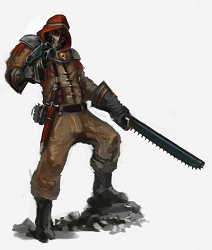
\includegraphics[width=\figwidth]{pics/4/17.png}
	\end{center}
\end{wrapfigure}
Thinking quickly Sarge had Alfred distract our Interrogator with a flask of tea while we formed a plan. 
Twitch would lead with some grenades, Sarge would flank left, Nubby and Doc would lay down covering fire, and Cutter would... run straight in screaming before any of us got into position.

Cutter's sudden charge caught us all off guard, it is a widely known fact that no guardsman has any business being closer to an Ork than the maximum range of their lasgun. 
Orks are bigger, stronger, and tougher than almost any soldier and they usually have a bunch of buddies nearby, despite all this the bloody psychopath was rushing straight into melee range of a whole squad of boyz. 
We did our best to lay down covering fire and watched in surprise as, instead of dying messily, Cutter began taking the greenskins apart. 

His new sword wrecked their choppas and his berserk fury surprised the hell out of the Orks. 
Limbs were flying, blood was everywhere, Gretchin were screaming, and not a single Ork noticed that we were mowing them down while they were busy, but it wasn't enough. 
The Orks began to overwhelm Cutter and we were sure that our melee specialist was going to be Squig food. 
Then, with a scream that perfectly matched Cutter's, another group of guardsmen rushed into the Orks from behind.

The fight was over in seconds and we all moved forward to greet the troopers who had saved Cutter. 
As we approached we noticed that each of them had a shiny new autogun, chainsword, and set of body armor; 
we had found the regiment.

\begin{wrapfigure}{O}{\figwidth}
	\begin{center}
		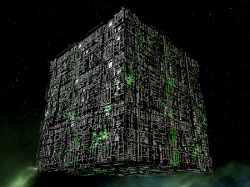
\includegraphics[width=\figwidth]{pics/4/18.png}
	\end{center}
\end{wrapfigure}
The walk to regiment's HQ was a little awkward. 
The troopers who escorted us were the biggest, ugliest, smelliest soldiers we had seen outside of the Ogryn auxiliaries and their accents were the worst we'd ever heard. 
Now, every world has its own variation of low gothic and several older regiments even have their own battle languages, so it wasn't unheard of for guardsmen from different regiments to have trouble talking to each other, but this was just ridiculous. 
It sounded like low gothic with half the letters missing, a lot of shouting, a bit of hitting, and a ridiculous amount of slang. 
We couldn't understand half of what they said and they didn't even try to understand us, it was lucky that Cutter had picked up their language somewhere and was able to act as a translator.

With Cutter's help we managed to convey that the Interrogator wanted to talk to their commander, that two 'friendly' convoys would be arriving shortly, and that we wanted to know where their guns came from.  
To our surprise this was accepted without fuss, there weren't any pointed questions, or evasions, or violent reactions. 
The Rupert, Cutter, and Alfred went off to talk to the regimental commander while the rest of us were taken to see what the troopers called The Box.

\begin{wrapfigure}{O}{\figwidth}
	\begin{center}
		
\includegraphics[width=\figwidth]{pics/4/19.png}
	\end{center}
\end{wrapfigure}
The Box was a huge pile of pipes, gears, screens, and other techy stuff; all crammed into a cube the size of a normal hab, which sat on a large flatbed in a warehouse. 
It had a big hopper on one end and a few conveyor belts coming out the other, as we watched a huge mess of scrap metal was dumped into the hopper by some of the troopers. 
A little while later a few of the new weapons rolled out on the belts and were collected by the troopers. 
The tech-priests were freaking out and yelling at each other in binary, we took this as a positive identification of The Box as the magos' gun factory.

We sat around and watched The Box for a bit while the adepts and tech-priests did their thing. 
Sarge and Doc speculated about the value of The Box and whether the odd behavior of the troopers was something sinister or not. 
To a man they were bigger and meaner looking than most guardsmen, the regiment was much farther forward than any sane guardsman would push, and they all seemed to be happy. 
Guardsmen are not supposed to be happy. 
Sarge was betting on some sort of daemon living in the box, Doc thought there might be some sort of heretical archeotech in there, Nubby didn't care, and Twitch had his own theory.

Twitch's paranoia had apparently gotten the better of him. 
He was interrupting every conversation to tell us that the troopers were Orks, and that the box was full of Orks, and that the Orks outside were double Orks.
Eventually we sent him to go secure us a base, the nerds said they couldn't concentrate with all his shouting.

\begin{wrapfigure}{O}{\figwidth}
	\begin{center}
		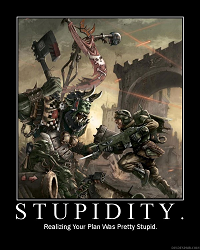
\includegraphics[width=\figwidth]{pics/4/20.png}
	\end{center}
\end{wrapfigure}
When the Interrogator returned from his little meeting and we brought him up to speed on The Box. 
Sarge and Doc shared their concerns about it being daemonic and corrupting the regiment, but the Rupert wouldn't hear a word of it. 
He maintained that the regiment was "positively spiffing; 
a splendid example of indomitable guardsman spirit" and that the regimental commander was "a jolly good fellow with just the right attitude for life in the guard, manners might need some polish though". 
The nerds and Alfred were no help, they all maintained that there was no warp corruption around The Box, though Alfred did admit it felt odd. As a last ditch effort Sarge convinced the Rupert to take a tour of the lines and watch the troopers in action.

So once again we split the party. 
Sarge, Cutter, Alfred, and the Interrogator went off to see how the troopers acted in combat while the rest of the team kept an eye on The Box.

The regiment was constantly fighting Orks so it was easy to find some action to watch. 
A section of the perimeter was currently taking fire from a group of Orks, and as they watched a full out assault was launched. 
Sarge was taking careful note of the troopers' discipline (poor), accuracy (abysmal), and attitude (excited), when he noticed that Cutter and the Rupert were missing. 
Both of them were rushing to reinforce the troopers' firing position before the Orks closed to melee. With a curse he and Alfred ran to catch up.

\begin{wrapfigure}{O}{\figwidth}
	\begin{center}
		
\includegraphics[width=\figwidth]{pics/4/21.png}
	\end{center}
\end{wrapfigure}
Sarge didn't have to worry though, before either of the idiots got to the barricade the troopers jumped out of cover and counter-charged. 
Autoguns in one hand and chainswords in the other, the troopers ran screaming into the onrushing Orks and everything devolved into a melee. 
Sarge and the Rupert stood on the barricade and watched in disbelief as more and more Orks and troopers ran to join the fight, both sides abandoning their positions for a chance to join the brawl. 
They were barely able to keep Cutter from running in too, if they hadn't all worked to restrain him he would have happily taken his new chainsword into the melee.

This was enough to convince the Interrogator that things were screwed up and The Box needed to go. 
Cutter was dragged away from the growing fight as they went to rejoin the team and see if blowing the source of the weapons to pieces fixed anything. 
Cutter calmed down as soon as he was away from the fight, but Sarge was pretty sure that the melee specialist was currently crazier than usual and started looking for a way to get the chainsword off of him without losing any fingers.
When they reached the warehouse they found it crawling with troopers.

With Cutter's help they talked their way inside where they found blood, bullet holes, several more troopers guarding The Box, and Twitch barricaded in the room he had been fortifying.

\begin{wrapfigure}{O}{\figwidth}
	\begin{center}
		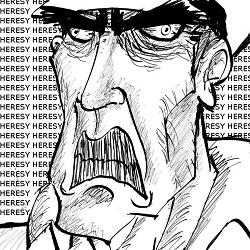
\includegraphics[width=\figwidth]{pics/4/22.png}
	\end{center}
\end{wrapfigure}
While Sarge and Cutter had been out spectating the rest of us had been chilling in the warehouse. 
Suddenly all of our coms went dead and one of the tech-priests helpfully informed us that we were being jammed. 
Not having anything better to do Doc and Nubby got directions towards the source of the jamming and left Twitch in charge of the nerds and The Box. 
Twitch did not feel this was important enough to merit leaving the room he was currently wiring with mines.

The source of the jamming turned out to be three chimeras with Commissariat markings that had just arrived. 
A single Commissar and a few squads of storm troopers were milling around trying to talk to the troopers and failing spectacularly. 
The second he saw the two guardsmen the Commissar and his goons marched over and ordered them to lead him to the source of the weapons.

This was a little unfair, we were in the Inquisition, we were supposed to be the guys that went around with storm troopers ordering people to do stuff they didn't want to do. 
Doc raised this point, but the Commissar was not inclined to take orders from a bunch of "jumped up guardsmen". 
When Doc tried to press the issue he got clubbed to the ground by one of the goons and Nubby decided that not having a concussion was the better part of valor.

Doc was left on the ground as Nubby led the Commissar and his men to The Box. 
Once they arrived the Commissar took one look at the box and made a terminal mistake; 
in nice loud voice he ordered his men to remove all the troopers from the room and rig The Box with explosives.

\begin{wrapfigure}{O}{\figwidth}
	\begin{center}
		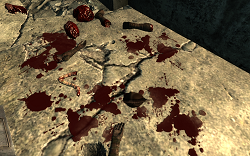
\includegraphics[width=\figwidth]{pics/4/23.png}
	\end{center}
\end{wrapfigure}
The second one of the goons tried to evict a trooper shit went south. 
The goon got decked, the Commissar shot the trooper, a few dozen more troopers rushed in, and things devolved into a general melee.
Nubby and the nerds took their chance and ran for Twitch's safe room, but the traps weren't quite finished and opening the door would’ve probably killed them all. 
So Nubby and the rest hid behind some rubble and watched as the Commissar and his goons were hacked to pieces by the enraged troopers.

The fight went on for a good while after the last of the Commissar's goons were dead, but eventually the troopers got tired and things quieted down. 
The corpses that littered the floor weren't just left there though, the troopers started gathering them up and dumping them into The Box where they were consumed with wet crunching sounds. 
This was a bit much for one of the adepts and before Nubby could restrain him the stupid bugger started screaming and praying. 
The troopers took notice of this and wandered over to the team's hiding spot.

Nubby immediately surrendered to the troopers and they were all led away by a big one with a whip. 
None of the troopers even checked the door that lead to Twitch's bolt-hole.

\begin{wrapfigure}{O}{\figwidth}
	\begin{center}
		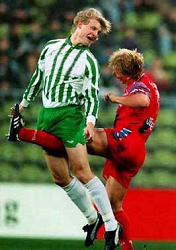
\includegraphics[width=\figwidth]{pics/4/24.png}
	\end{center}
\end{wrapfigure}
After all of this was relayed to Sarge and the Rupert it was decided that there would be no more splitting up. 
Twitch was pried out of his pile of explosives and trip wires and the whole group set out to find the rest of they set off to save the rest of the team. 
What followed was much more of scavenger hunt than a rescue mission.

The adepts were found first. 
They were both waist deep in a latrine pit with shovels while a bunch of troopers laughed and threw things at them. 
Cutter negotiated their release by kicking the largest trooper present in the crotch.

The tech-priests were in a nearby building helping a larger than usual trooper with a few augmetics weld entire chainswords onto autogun bayonet mounts. 
Cutter's negotiation tactic failed, it turned out the trooper's augmetics were a little more extensive than they had at first appeared. 
Luckily he was too busy laughing at Cutter's pain to notice when one of the tech-priests came up behind him and tased him.

Doc was found in the medical tent where a trooper in a smock was chasing him around with a circular saw and screaming about "fixing dat pesky brain". 
We skipped straight to the tasing this time, then went off to find Nubby.

To our surprise Nubby was in the command tent serving drinks and snacks to the regiment's officers and dodging the occasional kick. 
The officers were all huge men, by far the biggest we'd seen so far, but the Commander dwarfed them all. 
It took three sets of body armor kludged together to fit him, he was covered with weapons, and he had the Commissar's hat on his head. 

We weren't keen to try tasing him and having Cutter kick him in the junk was out of the question. 
So as tactfully as possible the Rupert greeted the Commander and offered to exchange a flask of his brandy for Nubby's release. 
To our relief he accepted. 
Reunited once more, we all headed for The Box to sort things out before one of the troopers snapped and we all got killed.

\begin{wrapfigure}{O}{\figwidth}
	\begin{center}
		
\includegraphics[width=\figwidth]{pics/4/25.png}
	\end{center}
\end{wrapfigure}
We immediately ran into problems when the troopers guarding the warehouse wouldn't let us in. 
A few arguments and blatant lies were tried, but the guards absolutely refused to stand aside. 
The Rupert started making plans for a glorious assault in which we would easily kill all the troopers, destroy The Box, then ride a tank of unspecified origin to safety. 
Sarge decided to go make his own plan.

It was Nubby's newfound status as regimental bitch that saved us from the Rupert's plan. 
While our Interrogator brainstormed with the nerds about where a unit of horse cavalry could be found for the victory parade, the rest of us did a little experimenting. 
We quickly discovered that as long as he was carrying a pile of junk taller than he was the guards would just ignore the greasy little soldier, only paying enough attention to throw a kick his way or lazily try to trip him. 
Seizing the initiative we stuck a pair of detpacks to a few pieces of scrap metal and sent our most cowardly squadmate to go destroy The Box and save the day.

\begin{wrapfigure}{O}{\figwidth}
	\begin{center}
		
\includegraphics[width=\figwidth]{pics/4/26.png}
	\end{center}
\end{wrapfigure}
Arms loaded with cargo Nubby waddled towards the warehouse entrance.
We all held our breath as one of the guards looked right at him, but all the trooper did was aim a lazy kick at Nubby's rear as he sidled past. 
We were all on pins and needles, ready to leap into action the second Nubby called for help, but the call never came. 
Instead after a few minutes Nubby sprinted back out as casually as he could manage. 

Right as he passed the guards one of them held out his foot and Nubby ate dirt. 
All the guards laughed as Nubby face planted and landed right on the detonator he was holding.

We all hit the dirt as an explosion shook the warehouse. 
Immediately afterwards we heard several smaller, wetter sounding explosions. 
As we rose out of cover to check on Nubby and the warehouse we were greeted by the sight of several headless guards slumping onto the ground. 
Sarge saluted the stunned Rupert, informed him that perimeter was clear, and requested further orders.

Not being men to look a gift horse in the mouth, or at least not this particular gift horse, we grabbed Nubby and followed our Interrogator into the warehouse to make sure The Box was completely destroyed. 
Inside we found several more headless troopers and one side of The Box blown open like a bag of popcorn. 
Weapons raised we slowly flanked around to get a look at what was inside, ready to face some daemonic monstrosity. 
It was full of Orks.

Twitch was so damn smug.

\begin{wrapfigure}{O}{\figwidth}
	\begin{center}
		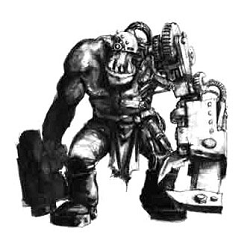
\includegraphics[width=\figwidth]{pics/4/27.png}
	\end{center}
\end{wrapfigure}
Well they weren't EXACTLY Orks, they looked more like Ork servitors, Servitorks. 
Regardless of what precisely they were, the second one saw us they let out a mighty 'Waaagh' and charged. 
We were ready for them though and the fact that most of them were still attached to The Box by tubes and cables slowed their pace significantly.

We poured las-fire into the Servitorks as they piled out of The Box. 
Fire discipline was maintained, targets were called out, and every soldier stood his ground;
unless you counted the adepts or tech-priests that is, they ran like little girls. 
We were bloody pros, it seemed like every shot we fired either killed or crippled, and the last Servitork collapsed a few feet short of a very disappointed Cutter.

We slowly advanced on the smoking hole in The Box, keeping an eye out for more surprises and, on Twitch's insistence, headshotting every single fallen Ork. 
When we reached the edge of the hole we all stopped. 
The Box was now filled with billowing smoke and random sparks, none of us guardsmen were eager to find out why. 

While we all stood around and debated the merits of walking into a smoking, xenos-powered, weapon dispenser, one of the tech-priests apparently found his balls.
He marched past us, head held high, and declared his intent to "return this relic to the bosom Omnissiah". 
A few seconds later there was a loud 'Zzap' and a smoking pile of metal sailed back out of the hole.

\begin{wrapfigure}{O}{\figwidth}
	\begin{center}
		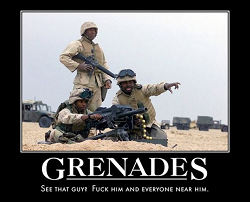
\includegraphics[width=\figwidth]{pics/4/28.png}
	\end{center}
\end{wrapfigure}
The Rupert let out an anguished shout and swore revenge, truly that cogboy had been a man among men and his like would never be seen again. 
He started a very moving speech about bravery, camaraderie, and charging into a box full of sparking smoke that was obviously hiding an Ork psyker.
While he did this we all popped frags and chucked them into The Box. 

We repeated this until we were out of frags, then waited until the smoke faded and revealed a partially slagged interior with a few smoldering Ork bits. 
The remaining tech-priest was none too happy with us and the Rupert seemed pretty put out that no one had wanted to charge into the smoke, but we didn't give a shit.
As far as we were concerned this was a job well done and the last thing to do was slap enough det packs onto the damned thing to make sure no one could ever fix it.

When we explained our plan to the rest of the team the remaining tech-priest called us a bunch of uneducated meatbags and stormed off. 
We ignored this and went to retrieve the munitions that Twitch had been wiring into his bolt-hole. 
This was not exactly a fast process and Twitch spent the entire time gloating, so everyone but Sarge went to go check the perimeter. 
Outside the warehouse the camp was absolute chaos; 
only the troopers near the warehouse had lost their heads, the rest of them just seemed to be very confused about just what the hell was going on.

The Rupert grabbed one of the panicking troopers and demanded a status report. 
In an entirely non-orky accent the soldier explained that the entire regiment had just realized that they were over extended, short on ammo, and had no defensive positions worth manning. 
The entire regiment was preparing to bug the hell out and get back to the main imperial lines, if we wanted to get out before the covering barrage hit we better get moving too. 
It felt damned good to hear that.

\begin{wrapfigure}{O}{\figwidth}
	\begin{center}
		
\includegraphics[width=\figwidth]{pics/4/29.png}
	\end{center}
\end{wrapfigure}
We were all congratulating ourselves, grabbing well-earned smokes, and watching Twitch work when the tech-priest returned. 
He made a very passionate sounding plea for returning The Box to the ad-mech for study. 
His completely monotone voice was overflowing with emotion and it melted our icy guardsman hearts, how could we stand in the way of science and deprive the mechanicus of what was practically a holy relic? 
With tears in his eyes Sarge told the tech-priest that he could take home all the scraps he could carry after we blew the damned thing to shrapnel. 
For some reason this didn't go over well.

There was a lot of shouting, some unkind things were said, and eventually the Rupert came over to see what all the fuss was about. 
We explained the situation and the tech-priest made his case for taking the mind altering, xenos powered box of horrors home with him and presumably marrying it since he loved the damned thing so much. 
Luckily our Interrogator came down on the side of reason. 
He very politely told the cogboy that this idea was incredibly stupid, and by extension so was the cogboy for even thinking it. 
This was the final straw for the tech-priest, he screeched something in binary and metal claws ripped through one of the warehouse's doors. 
Apparently the Mechanicus convoy had finally arrived.

\begin{wrapfigure}{O}{\figwidth}
	\begin{center}
		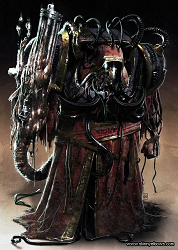
\includegraphics[width=\figwidth]{pics/4/30.png}
	\end{center}
\end{wrapfigure}
The senior magos of the local ad-mech detachment, the one who had been arguing with us about proper ownership of the weapons during the investigation, tore through the doors and he was a lot bigger than we remembered. 
When we had initially dealt with the magos he had looked like a normal tech-priest, he'd apparently decided to go get a few combat augmetics for his trip to the front. 
Being guardsmen we all firmly believed that there was no such thing as overkill, but this was damned close; 
there were probably smaller dreadnaughts out there. 
He stomped in with a few servitors backing him up and calmly asked the Rupert to reconsider.

A sane man might have seen the folly of arguing with a three meter tall pile of guns and mechadendrites, but not our Interrogator. 
In his mind there was no way he could be wrong; 
anyone who disagreed was either unbelievably stupid or doing it just to spite him, therefore it was his job to either educate them or win them over with his gentlemanly charm. 
While we all stood back and tried to look non-threatening the poor bastard did his damnedest to explain the way the universe was supposed to work to an increasingly annoyed magos. % TYPO damndest to damnedest
When this failed he tried to appeal to the humanity of a creature that was more closely related to a Leman Russ than the average human being. 
When that inevitably failed the Rupert gave in to his frustration, drew his sword, and challenged the metal monstrosity to a duel.

The magos responded by tasing him.

\begin{wrapfigure}{O}{\figwidth}
	\begin{center}
		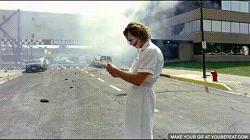
\includegraphics[width=\figwidth]{pics/4/31.png}
	\end{center}
\end{wrapfigure}
Tasing probably isn't the right term. 
For one thing most tasers aren't tesla coils mounted on the end of a metal tentacle, also tasing doesn't usually involve a ten foot bolt of lightning that melts swords or chars arms to the bone. 
It sure as hell incapacitated the Rupert though. 

That was enough to convince us that we wanted no part of this shit. 
While Alfred and Doc saw to our slightly over-cooked Interrogator Sarge formally surrendered The Box to the magos and had Twitch hand over the detonator to the explosives he had covered the box with. 
We bid farewell to the magos and the little shit-stain of a tech-priest then made our way to the exit. 
As we left we watched the two cogboys, practically oiling their pants in delight, walked up to The Box then reverentially entered it through the hole we had blasted.

Then Twitch hit the trigger on his backup detonator.

Seriously, who doesn't set up redundant detonators when they're doing demolition work? 
It's not like you want to walk up and try to fix it if your detonator fails. 
Some people are just so stupid.

\begin{wrapfigure}{O}{\figwidth}
	\begin{center}
		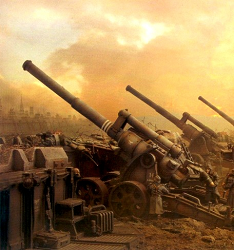
\includegraphics[width=\figwidth]{pics/4/32.png}
	\end{center}
\end{wrapfigure}
We made our way to the Chimeras the Commissar had used to get here and requisitioned a few drivers from the regiment.
The trip back was much less eventful than the trip out, half a regiment had just been through the area and no Gretchin is dumb enough to take pot-shots at a Chimera. 
Sarge used the vehicle's vox to call HQ and get them to walk the covering barrage over the regiment's former position after the retreat was finished. 
Sure we had reduced the two tech-priests and their box to greasy stains on the ground, but there was no harm in making sure.

We rode back to HQ with the comforting sound of IG artillery in our ears.

\begin{wrapfigure}{O}{\figwidth}
	\begin{center}
		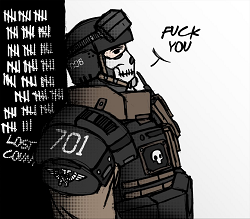
\includegraphics[width=\figwidth]{pics/4/33.png}
	\end{center}
\end{wrapfigure}
Sarge delivered the team's report to the Generals and the other big wigs since the Rupert was doped to the eyeballs on painkillers.
We gave the regiment and the remaining weapons a clean bill of health, after The Box and its weirdboy had been dealt with the weapons had stopped being supernaturally awesome and the troopers had stopped acting like Orks. 
All that remained was some perfectly normal gear and some unusually buff soldiers.

We pinned the death of the Commissar and his storm troopers on the Orks, it was more or less true anyway. 
The Commissariat wasn't exactly happy with this explanation, but they blamed us instead of the troopers and we were already on our way off planet, so we didn’t worry too much. 
The Mechanicus was also pretty pissed about the destruction of The Box, unfortunately their boss had mysteriously gone missing during the retreat and they didn't have the authority to really do anything about it. 
We suggested that both groups lodge a formal complaint with Oak.

With the help of Alfred we requisitioned a berth on a navy ship going our way then got the hell off that planet before the Commissariat or Mechanicus tried to kill us.

\begin{wrapfigure}{O}{\figwidth}
	\begin{center}
		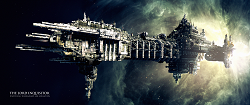
\includegraphics[width=\figwidth]{pics/4/34.png}
	\end{center}
\end{wrapfigure}
The ride back to Professor Oak's Spacefaring Inquisitorial Doom School was relaxing. 
Doc got to learn about augmetic shoulder sockets and even helped a navy surgeon install one on the Rupert. 
Nubby and Cutter played around with the weapons and gear they had looted. 
Sarge helped Alfred write the final report and enjoyed the fact that the adepts were too scared to talk to him now. 
Twitch gloated like a dog that caught a squirrel.

Every conversation with him started with "Remember how I said it was Orks and you all called me crazy?".
There's nothing quite as annoying as a paranoid who's been proved right.

Eventually we got back to Oak's ship, delivered our report and wandered back down to our little section, it was good to be home. 
A few days later, well before we could get into the proper spirit of R\&R, a runner came for us with orders to report to Oak's office. 
We all thought back to when we told the ad-mech and Commissariat to file a complaint and desperately hoped that Oak wasn't about to turn us all over as a gesture of goodwill.

\begin{wrapfigure}{O}{\figwidth}
	\begin{center}
		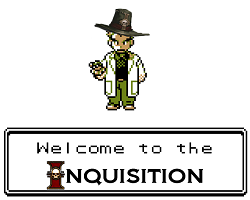
\includegraphics[width=\figwidth]{pics/4/35.png}
	\end{center}
\end{wrapfigure}
Sarge's fears were unfounded though, after the rest of the team arrived Oak praised us all for our exceptional performance. 
He congratulated the Interrogator especially for identifying the root cause of the problem, removing a piece of heretical technology, and handling the political situation without launching a massive and wasteful purge (Sarge had to kick Twitch when "identifying the root cause" was mentioned). 
After he finished praising us and lamenting the treachery of the tech-priest, Oak presented a rosette to the Rupert and welcomed him as a full member of the Ordos. 
To our considerable surprise the Rupert turned the promotion down.

With tears in his eyes and a choke in his voice the Rupert explained that while Oak was happy with our team's performance, he was not satisfied with his own personal performance on the mission. 
He gave a heartfelt speech about the importance of looking out for your men, listening to their advice (Twitch got another kick here), and not taking foolish personal risks like challenging giant metal men to duels. 
We only understood three words in ten, but it was very touching nonetheless.

He ended the speech with a request that Oak let him take the exam again after he got a new augmetic arm. 
A rather bemused Oak agreed and dismissed us all. 
As we left the Rupert thanked us for our valiant service and promised to request us for his team once he had recovered. 
We weren't sure how we felt about that, he wasn't perfect but were definitely worse interrogators out there.

\begin{wrapfigure}{O}{\figwidth}
	\begin{center}
		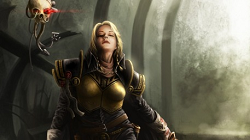
\includegraphics[width=\figwidth]{pics/4/36.png}
	\end{center}
\end{wrapfigure}
Once that drama was over with we all went and enjoyed our downtime as only guardsman on leave can. 
There's an old guard saying that goes "Life is short, party hard". 

Our R\&R ended far too soon, we all still had money and functioning brain cells when the runner came for us. 
Sarge got us all into the suits Alfred had gotten us and looking far too spiffy we marched ourselves onto the waiting shuttle.

The most beautiful woman we had ever seen greeted us and told us to stand easy. 
Then, with a smile that would have made the Emperor himself blush, she asked us what we knew about genestealers. 

Sarge barely managed to catch Nubby and Twitch as they bolted for the shuttle hatch.



